\section{Numerical experiments}

\begin{frame}
  \frametitle{Simulation study: settings}

  \begin{enumerate}
\item  Draw a $p \times p$ adjacency matrix $\bA$ under Erd\"os-Renyi model.
\item  Expand $\bA$  to  multivariate space: 
  $$\mathbf{M} = \mathbf{A}  \otimes \mathbb{S} + \mathbf{I}_{p\times K}$$
  \paragraph{$\mathbb{S}$ is used to consider different scenarios of agreement}
  \begin{enumerate}[a)]
  \item $\mathbb{S} = \mathbf{I}_{K,K}$ \\ 
    \rsa same intra-attribute network, no inter-attribute interactions
  \item $\mathbb{S} = \mathbf{I}_{K,K} - \mathbf{1}_{K,K}$ \\ 
  \rsa same inter-attribute interactions and no intra-attribute interactions
  \item $\mathbb{S} = \mathbf{1}_{K,K}$ \\
    \rsa full agreement between  attributes.
  \end{enumerate}
\item $\invcov$ is the nearest a positive definite approximation of $\mathbf{M}$
\item Control the difficulty with $\gamma>0: \invcov= \invcov+ \gamma I$;
\item Draw an i.i.d. $n$-size sample $\bX\in\Rset^{n\times pK}$ of
  $X \sim \mathcal{N} \left( 0,\invcov^{-1} \right) .$
\end{enumerate}


\end{frame}

\begin{frame}
  \frametitle{Simulation study: evaluation}

  \begin{block}{Competitors}  
  \begin{itemize}
  \item \texttt{multiattribute}: reconstruct one network with
   $K$ data sets $\bX^{(1)}, \dots \bX^{(K)}$ all with size
  $\Rset^{n\times p}$

  \item \texttt{separate}: reconstruct $K$ networks with
   $K$ data sets $\bX^{(1)}, \dots \bX^{(K)}$ all with size
  $\Rset^{n\times p}$

  \item the \texttt{merge} variant: reconstruct one network 
    by merging $\bX^{(1)}, \dots \bX^{(K)}$ into a single
    $\tilde\bX$ data set in $\Rset^{nK \times p}$
  \end{itemize}
  \end{block}
  
  \begin{block}{Performances}  
    Use area under ROC curve (AUC). For the \textit{separate} variant, the retained AUC is the AUC
    averaged over all attributes.  
  \end{block}

  \rsa Set $p=40$, vary $n, K$ and replicate 100 times

\end{frame}


\begin{frame}
  \frametitle{Simulation study: results}
  
  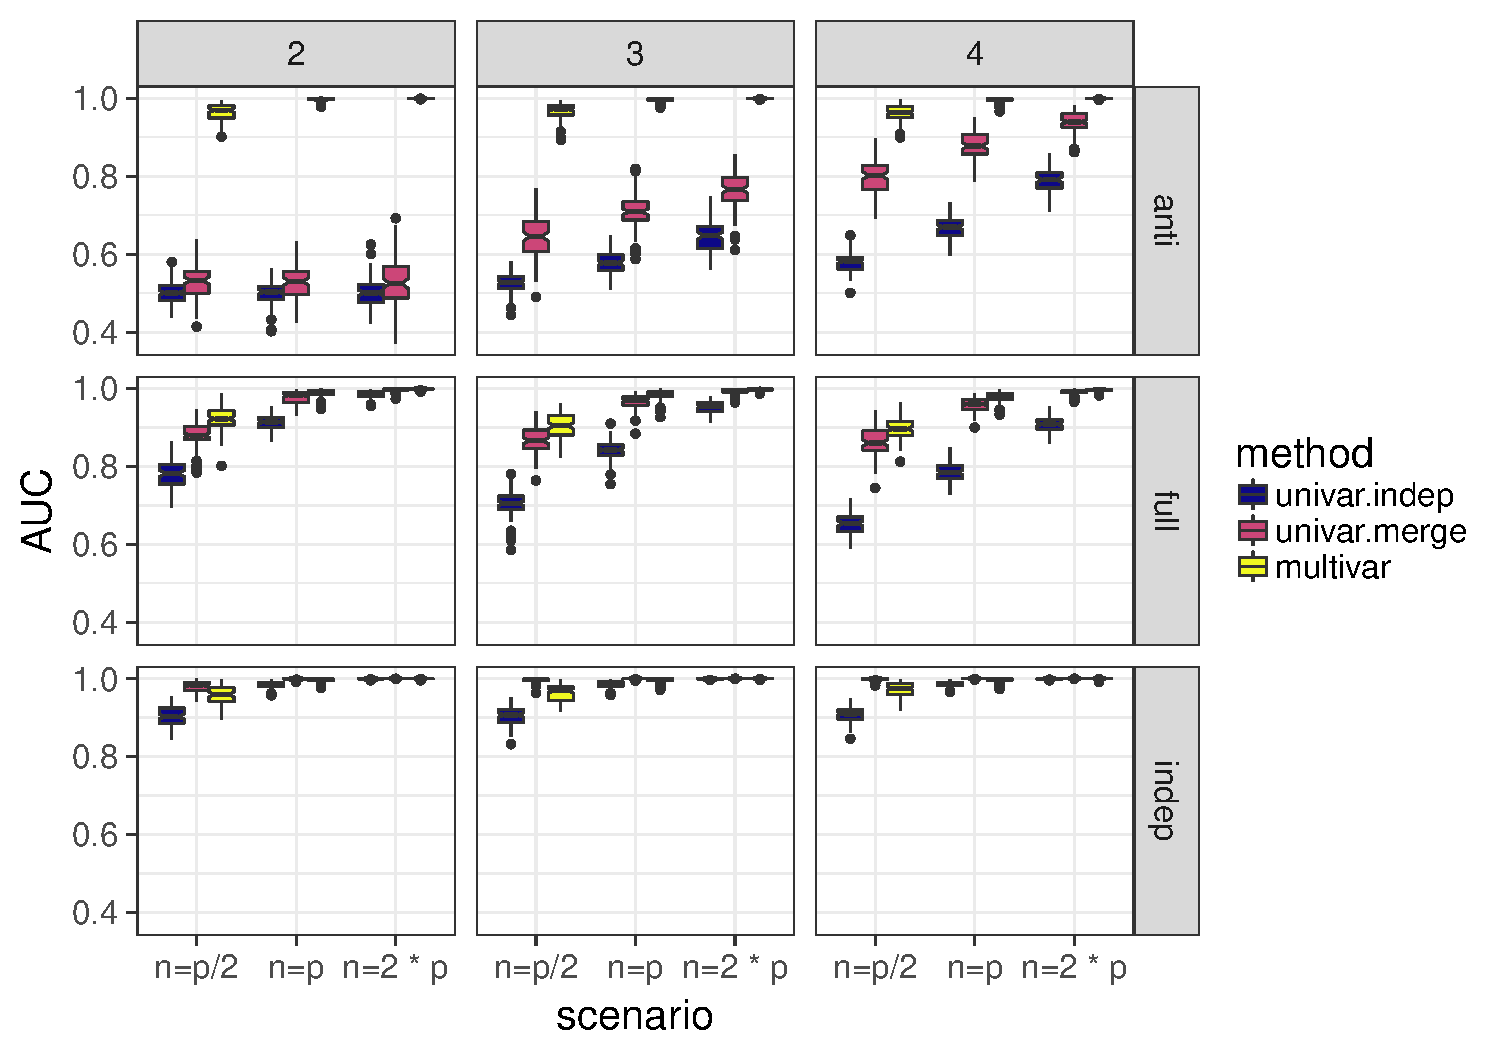
\includegraphics[width=\textwidth]{../../chapter/figures/res_simu_new}

\end{frame}
